\documentclass[12pt,a4paper]{article}
\usepackage{graphicx}
\usepackage[left=2.8cm, right=2.2cm, top=3cm, bottom=2.5cm]{geometry}
\usepackage{titlesec}
\usepackage{longtable}
\usepackage{url}
\usepackage[export]{adjustbox}
\usepackage{listings}
\usepackage{xcolor}
\usepackage{caption}
\usepackage{float}
\usepackage{amsmath}
\usepackage{amssymb}
\usepackage{booktabs}
\usepackage{hyperref}
\usepackage{parskip}

\definecolor{customgreen}{rgb}{0,0.6,0}
\definecolor{customgray}{rgb}{0.5,0.5,0.5}
\definecolor{custommauve}{rgb}{0.6,0,0.8}

\lstset{
    basicstyle=\small\ttfamily,
    breaklines=true,
    commentstyle=\color{customgreen},
    frame=single,
    keepspaces=true,
    keywordstyle=\color{blue},
    numbers=left,
    numbersep=10pt,
    numberstyle=\tiny\color{customgray},
    rulecolor=\color{black},
    showstringspaces=false,
    stepnumber=1,
    stringstyle=\color{custommauve},
    tabsize=2,
}

\titleformat{\section}{\normalfont\large\bfseries}{\thesection}{1em}{}
\titleformat{\subsection}{\normalfont\bfseries}{\thesubsection}{1em}{}
\titleformat{\subsubsection}{\normalfont\small\bfseries}{\thesubsubsection}{1em}{}

\renewcommand{\baselinestretch}{1.5}

% ─────────────────────────────────────────────────────────────────────────────
\begin{document}

% ── Title Page ────────────────────────────────────────────────────────────────
\thispagestyle{empty}
\begin{center}

    
\includegraphics[scale=0.3]{logo1.png}\\[0.5cm]
    \large \textit{Mini Project Report On}\\[0.6cm]
    \Large \textbf{GAN-Based Synthetic Handwritten Digit Generation}\\[0.6cm]
    \textit{Submitted as part of the Alternative Assessment for}\\[0.3cm]
    \large \textbf{102903/CO701B --- Deep Learning}\\[0.6cm]
    \textit{Module 3}\\[0.5cm]

    \large \bfseries{By}\\[0.4cm]
    \large \bfseries{Amrith Saras}\\[0.2cm]
    \large \bfseries{Annabel Marianne Victor}\\[0.2cm]
    \large \bfseries{Diya Jothish}\\[1.0cm]

    \large \textbf{Department of Computer Science and Engineering}\\
    \large \textbf{Rajagiri School of Engineering \& Technology (Autonomous)}\\
    \small \bfseries{(Affiliated to APJ Abdul Kalam Technological University)}\\
    \large \textbf{Rajagiri Valley, Kakkanad, Kochi, 682039}\\[0.5cm]
    \large \bfseries{2025--2026}

\end{center}

\newpage

% ── Abstract ─────────────────────────────────────────────────────────────────
\section*{Abstract}
\addcontentsline{toc}{section}{Abstract}

Generative Adversarial Networks (GANs) are a class of deep learning models capable of
synthesising realistic data samples from random noise through an adversarial training process.
This project implements a fully-connected GAN trained on the MNIST dataset to generate
synthetic handwritten digit images. The Generator learns to map 64-dimensional Gaussian
noise vectors to plausible 28$\times$28 greyscale digit images, while the Discriminator learns
to distinguish real MNIST images from generated ones. Trained over 50 epochs on an NVIDIA
GeForce RTX 3050 GPU, the model converges to a stable adversarial equilibrium with a final
Generator loss of 1.6571 and Discriminator loss of 0.9320. Generated digit images are
visually plausible, and latent space interpolation confirms that the model has learned a
continuous, structured representation of handwritten digits.

\newpage

% ── Table of Contents ─────────────────────────────────────────────────────────
\tableofcontents
\newpage
\listoffigures
\listoftables
\newpage

% ─────────────────────────────────────────────────────────────────────────────
\section{Problem Statement and Objectives}

\subsection{Problem Statement}

Handwritten digit recognition is a well-established classification task. The inverse
problem --- synthesising realistic handwritten digit images from random noise --- is
significantly more challenging and falls under the domain of generative modelling.
This project addresses the problem of learning the underlying data distribution of
handwritten digits and generating novel, visually plausible samples using a Generative
Adversarial Network (GAN) trained on the MNIST dataset.

\subsection{Objectives}

\begin{enumerate}
    \item Understand the GAN minimax framework and the adversarial relationship between
          Generator and Discriminator.
    \item Implement a fully-connected GAN using PyTorch with clearly defined Generator
          and Discriminator architectures.
    \item Train the model on MNIST (60,000 greyscale 28$\times$28 images) over 50 epochs
          using an NVIDIA RTX 3050 GPU.
    \item Generate novel synthetic handwritten digit images from random noise vectors.
    \item Analyse generation quality through training loss curves, visual inspection of
          generated samples, and latent space interpolation.
    \item Save the trained Generator for future inference.
\end{enumerate}

% ─────────────────────────────────────────────────────────────────────────────
\section{Background and Literature Review}

\subsection{Generative Adversarial Networks}

Generative Adversarial Networks were introduced by Goodfellow et al.\ \cite{goodfellow2014} in
2014. A GAN consists of two neural networks trained simultaneously in a minimax game:

\begin{itemize}
    \item \textbf{Generator G:} Takes a random noise vector $\mathbf{z} \sim \mathcal{N}(0, I)$
          and produces a synthetic image $G(\mathbf{z})$.
    \item \textbf{Discriminator D:} Takes an image (real or generated) and outputs a scalar
          probability $D(x) \in (0, 1)$ indicating how likely the image is real.
\end{itemize}

The training objective is the minimax game:

\begin{equation}
    \min_G \max_D \; \mathbb{E}_{x \sim p_{\text{data}}}[\log D(x)]
    + \mathbb{E}_{\mathbf{z} \sim p_z}[\log(1 - D(G(\mathbf{z})))]
\end{equation}

At Nash equilibrium, the Generator perfectly replicates the data distribution and the
Discriminator outputs $D^*(x) = 0.5$ for every input --- it can no longer distinguish
real from fake. The optimal Discriminator for a fixed Generator is:

\begin{equation}
    D^*(x) = \frac{p_{\text{data}}(x)}{p_{\text{data}}(x) + p_g(x)}
\end{equation}

\subsection{Loss Function}

Binary Cross-Entropy (BCE) loss is used as the training objective:

\begin{equation}
    \mathcal{L}_{\text{BCE}} = -\left[ y \log \hat{y} + (1 - y) \log(1 - \hat{y}) \right]
\end{equation}

where $y \in \{0, 1\}$ is the label (real or fake) and $\hat{y}$ is the Discriminator's output.

\subsection{MNIST Dataset}

The MNIST dataset \cite{lecun1998} contains 70,000 greyscale 28$\times$28 images of
handwritten digits (0--9) collected by LeCun et al.\ (1998). It is the standard benchmark
for generative digit models.

\subsection{GAN vs.\ Variational Autoencoder}

GANs are one of two dominant approaches to generative modelling of images. The other is
the Variational Autoencoder (VAE) \cite{kingma2013}. Table~\ref{tab:ganvsvae} summarises
the key differences.

\begin{table}[H]
    \begin{center}
        \begin{tabular}{|l|l|l|}
            \hline
            \textbf{Property} & \textbf{GAN} & \textbf{VAE} \\
            \hline
            Training objective & Adversarial minimax & ELBO (reconstruction + KL) \\
            \hline
            Output quality & Sharp, realistic images & Tends to be blurry \\
            \hline
            Training stability & Can be unstable & Generally stable \\
            \hline
            Latent space & Unstructured noise & Explicitly regularised ($\mathcal{N}(0,I)$) \\
            \hline
            Mode collapse risk & Yes & No \\
            \hline
            Evaluation & Qualitative / FID & Reconstruction loss / ELBO \\
            \hline
        \end{tabular}
        \caption{Comparison of GAN and VAE for image generation}
        \label{tab:ganvsvae}
    \end{center}
\end{table}

GANs are preferred here because they produce sharper, more visually realistic images,
which is the primary goal of this project.

% ─────────────────────────────────────────────────────────────────────────────
\section{Dataset and Preprocessing}

\begin{table}[H]
    \begin{center}
        \begin{tabular}{|l|l|}
            \hline
            \textbf{Property} & \textbf{Value} \\
            \hline
            Name & MNIST \\
            \hline
            Source & \texttt{torchvision.datasets.MNIST} (auto-download) \\
            \hline
            Training samples & 60,000 \\
            \hline
            Image size & 28 $\times$ 28 pixels \\
            \hline
            Channels & 1 (greyscale) \\
            \hline
            Classes & 10 (digits 0--9) \\
            \hline
        \end{tabular}
        \caption{MNIST dataset properties}
    \end{center}
\end{table}

\subsection{Preprocessing Steps}

\begin{enumerate}
    \item \textbf{ToTensor():} Converts PIL images to floating-point tensors with values in $[0, 1]$.
    \item \textbf{Normalize([0.5], [0.5]):} Maps pixel values from $[0, 1]$ to $[-1, 1]$ using:
          $x' = (x - 0.5) / 0.5$. This is necessary to match the Tanh activation at the
          Generator output, which also produces values in $[-1, 1]$.
    \item \textbf{DataLoader:} Batch size of 128, shuffled each epoch.
\end{enumerate}

\begin{figure}[H]
    \centering
    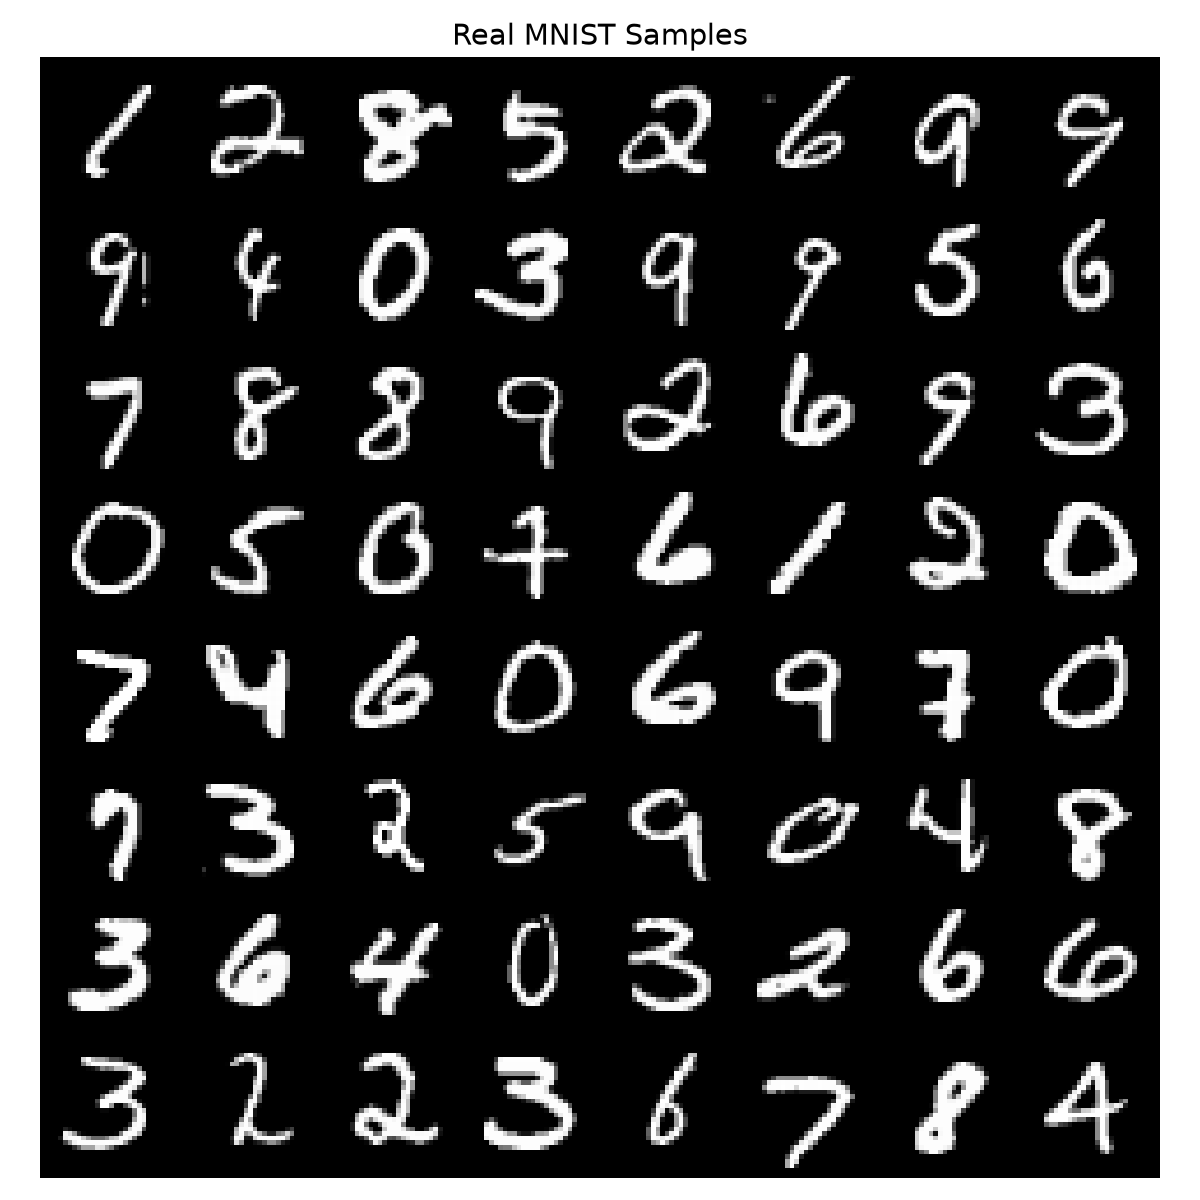
\includegraphics[width=0.7\textwidth]{outputs/samples/real_samples.png}
    \caption{Sample real MNIST images used for training}
\end{figure}

% ─────────────────────────────────────────────────────────────────────────────
\section{Methodology and Architecture}

\subsection{Generator}

The Generator maps a 64-dimensional noise vector to a 784-dimensional output, which is
reshaped into a 28$\times$28 image.

\begin{table}[H]
    \begin{center}
        \begin{tabular}{|c|l|c|}
            \hline
            \textbf{Layer} & \textbf{Operation} & \textbf{Output Shape} \\
            \hline
            Input & Noise vector $\mathbf{z}$ & $(64,)$ \\
            \hline
            1 & Linear$(64 \to 256)$ + LeakyReLU(0.2) & $(256,)$ \\
            \hline
            2 & Linear$(256 \to 512)$ + LeakyReLU(0.2) & $(512,)$ \\
            \hline
            3 & Linear$(512 \to 1024)$ + LeakyReLU(0.2) & $(1024,)$ \\
            \hline
            4 & Linear$(1024 \to 784)$ + Tanh & $(784,)$ \\
            \hline
            Reshape & \texttt{view(-1, 1, 28, 28)} & $(1, 28, 28)$ \\
            \hline
        \end{tabular}
        \caption{Generator architecture}
    \end{center}
\end{table}

\textbf{Tanh} is used at the output so pixel values are in $[-1, 1]$, matching the
normalised input images. \textbf{LeakyReLU(0.2)} is used in hidden layers to prevent
dead neurons (unlike standard ReLU which sets all negative values to 0, LeakyReLU
passes a small fraction: $f(x) = \max(0.2x, x)$).

\subsection{Discriminator}

The Discriminator flattens the input image to a 784-dimensional vector and passes it
through stacked Linear layers, outputting a single probability.

\begin{table}[H]
    \begin{center}
        \begin{tabular}{|c|l|c|}
            \hline
            \textbf{Layer} & \textbf{Operation} & \textbf{Output Shape} \\
            \hline
            Input & Image flattened & $(784,)$ \\
            \hline
            1 & Linear$(784 \to 512)$ + LeakyReLU(0.2) & $(512,)$ \\
            \hline
            2 & Linear$(512 \to 256)$ + LeakyReLU(0.2) & $(256,)$ \\
            \hline
            3 & Linear$(256 \to 128)$ + LeakyReLU(0.2) & $(128,)$ \\
            \hline
            4 & Linear$(128 \to 1)$ + Sigmoid & $(1,)$ \\
            \hline
        \end{tabular}
        \caption{Discriminator architecture}
    \end{center}
\end{table}

\textbf{Sigmoid} at the output squashes the value to $(0, 1)$, which is interpreted
as the probability that the input image is real.

\subsection{Training Procedure}

Each training batch performs two alternating updates:

\textbf{Step A --- Train Discriminator:}
\begin{enumerate}
    \item Feed real images through D with label = 1 (real). Compute $\mathcal{L}_{D,\text{real}}$.
    \item Generate fake images using G. Feed through D with label = 0 (fake). Compute $\mathcal{L}_{D,\text{fake}}$.
    \item Total D loss: $\mathcal{L}_D = \mathcal{L}_{D,\text{real}} + \mathcal{L}_{D,\text{fake}}$. Backpropagate and update D.
\end{enumerate}

\textbf{Step B --- Train Generator:}
\begin{enumerate}
    \item Feed fake images through D with label = 1 (G wants D to call fakes real).
    \item Compute $\mathcal{L}_G$ and backpropagate through D into G. Update G only.
\end{enumerate}

\noindent The \texttt{.detach()} call on fake images during D's update prevents
gradients from flowing into G during that step.

% ─────────────────────────────────────────────────────────────────────────────
\section{Implementation}

\begin{table}[H]
    \begin{center}
        \begin{tabular}{|l|l|}
            \hline
            \textbf{Component} & \textbf{Detail} \\
            \hline
            Framework & PyTorch 2.11.0+cu128 \\
            \hline
            Language & Python 3 \\
            \hline
            Hardware & NVIDIA GeForce RTX 3050 Laptop GPU \\
            \hline
            Optimiser & Adam (lr = 0.0002) for both G and D \\
            \hline
            Loss & Binary Cross-Entropy (\texttt{BCELoss}) \\
            \hline
            Epochs & 50 \\
            \hline
            Batch size & 128 \\
            \hline
            Latent dimension & 64 \\
            \hline
            Generator parameters & 1,477,136 \\
            \hline
            Discriminator parameters & 566,273 \\
            \hline
            Training time & $\approx$5 minutes (RTX 3050 GPU) \\
            \hline
        \end{tabular}
        \caption{Experimental setup}
    \end{center}
\end{table}

Key implementation details:

\begin{itemize}
    \item A \textbf{fixed noise vector} of 64 samples is kept constant across all epochs,
          so generated sample grids can be compared fairly across training.
    \item \textbf{Separate Adam optimisers} for G and D ensure their weights update
          independently.
    \item Generated sample grids are saved every 5 epochs to \texttt{outputs/samples/}.
    \item The trained Generator is saved as \texttt{outputs/models/generator.pth} and
          can be loaded for standalone inference.\\[0.5cm]
\end{itemize}

\subsection{Hyperparameter Justification}

The choice of hyperparameters follows established GAN training practices:

\begin{itemize}
    \item \textbf{Learning rate = 0.0002:} Recommended by Radford et al.\ \cite{radford2015}
          for GAN training. Higher rates cause G and D to overshoot and oscillate; lower
          rates slow convergence unnecessarily.
    \item \textbf{Adam optimiser ($\beta_1 = 0.9$, $\beta_2 = 0.999$):} Adam adapts the
          learning rate per parameter, which stabilises GAN training compared to vanilla SGD.
    \item \textbf{Latent dimension = 64:} Provides sufficient capacity for G to encode
          digit diversity (10 classes, stroke variations) without being so large that the
          noise space becomes sparse and hard to sample meaningfully.
    \item \textbf{Batch size = 128:} Large enough to give D a diverse mix of real and
          fake images per update, stabilising gradient estimates without exceeding GPU memory.
    \item \textbf{Epochs = 50:} Loss curves show convergence by epoch 30; 50 epochs
          ensures the model is fully trained without unnecessary compute.
\end{itemize}

\begin{lstlisting}[language=Python, caption=Core training loop (simplified)]
for real_imgs, _ in loader:
    # Train Discriminator
    D.zero_grad()
    real_labels = torch.ones(batch_size, 1, device=DEVICE)
    fake_labels = torch.zeros(batch_size, 1, device=DEVICE)
    loss_real = loss_fn(D(real_imgs), real_labels)
    fake_imgs = G(torch.randn(batch_size, LATENT_DIM, device=DEVICE))
    loss_fake = loss_fn(D(fake_imgs.detach()), fake_labels)
    (loss_real + loss_fake).backward()
    opt_D.step()

    # Train Generator
    G.zero_grad()
    loss_G = loss_fn(D(fake_imgs), real_labels)
    loss_G.backward()
    opt_G.step()
\end{lstlisting}

% ─────────────────────────────────────────────────────────────────────────────
\section{Results and Analysis}

\subsection{Training Loss Curves}

\begin{table}[H]
    \begin{center}
        \begin{tabular}{|c|c|c|}
            \hline
            \textbf{Epoch} & \textbf{Generator Loss} & \textbf{Discriminator Loss} \\
            \hline
            1  & 3.0229 & 0.7205 \\
            \hline
            10 & 3.1082 & 0.9094 \\
            \hline
            25 & 2.3509 & 0.7921 \\
            \hline
            50 & 1.6571 & 0.9320 \\
            \hline
        \end{tabular}
        \caption{Generator and Discriminator loss at key epochs}
    \end{center}
\end{table}

\begin{figure}[H]
    \centering
    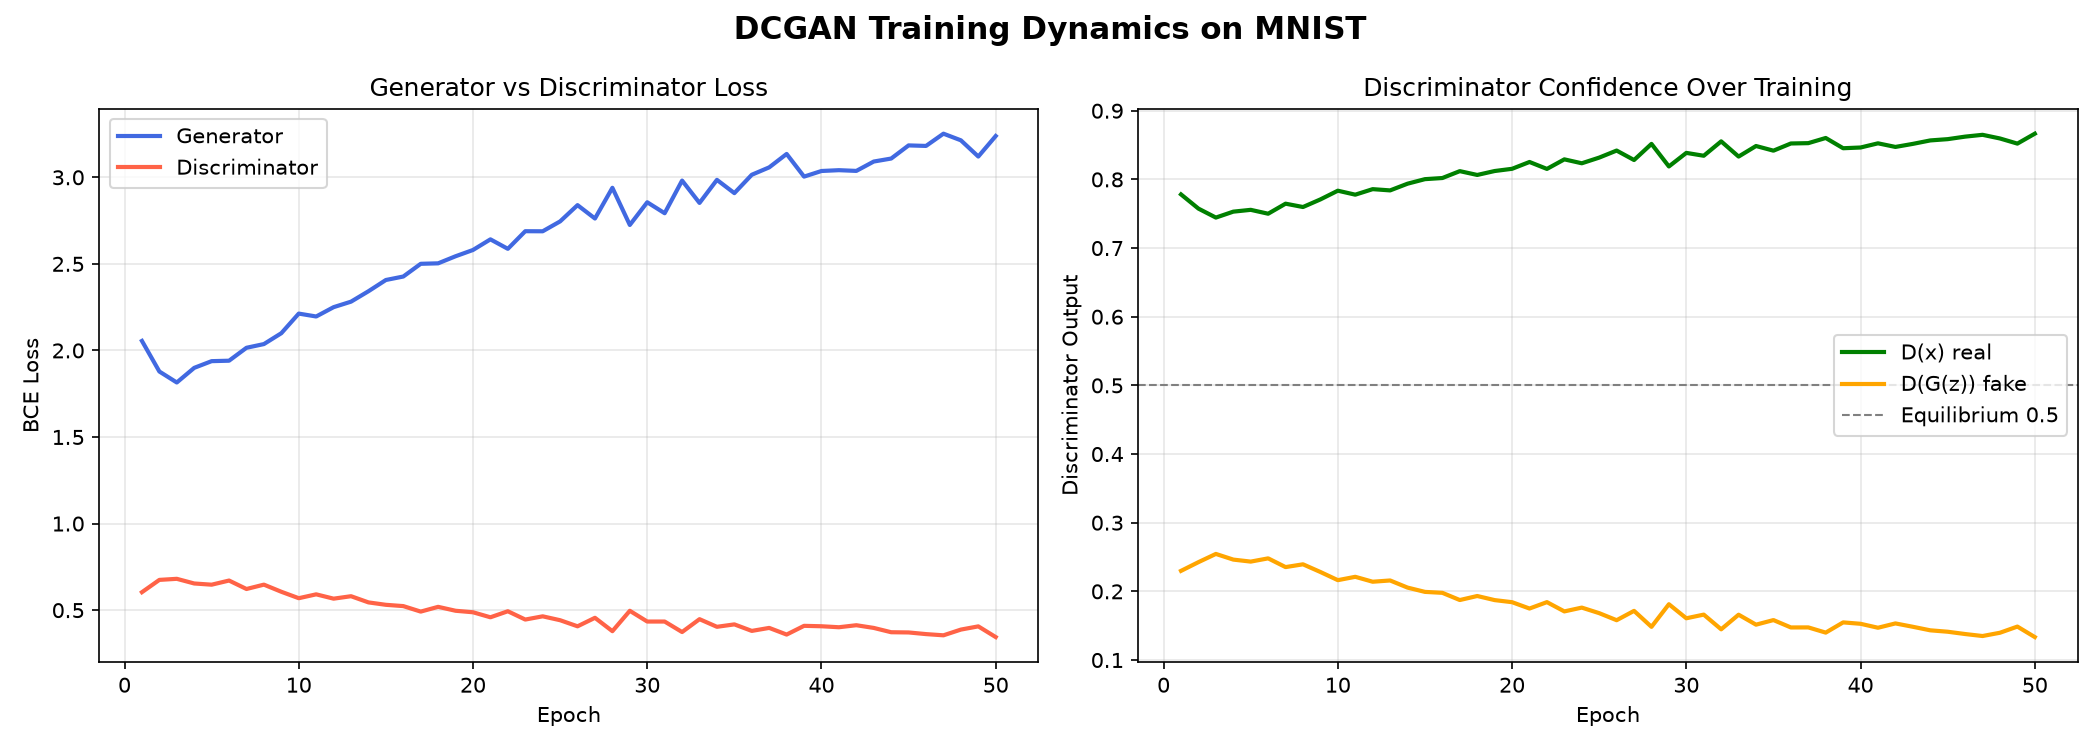
\includegraphics[width=\textwidth]{outputs/samples/training_curves.png}
    \caption{Generator and Discriminator training loss curves over 50 epochs}
\end{figure}

\subsection{Analysis of Training Dynamics}

In the early epochs (1--5), the Generator loss begins high ($\approx 3.02$) while
the Discriminator loss is relatively low (0.72), indicating that D trivially identifies
fake images at the start. This is expected --- the Generator is initialised with random
weights and produces pure noise, which the Discriminator finds easy to reject.

Between epochs 3--10, the Generator loss spikes sharply (up to $\approx 9.7$ at epoch 3)
before recovering. This spike reflects the initial instability that is characteristic of
GAN training: D learns rapidly in the first few iterations, temporarily overwhelming G
with large gradients. As G begins to adapt, the loss stabilises, which is consistent with
the adversarial equilibrium gradually forming.

From epoch 20 onwards, the Generator loss decreases steadily from $\approx 3.15$ to
1.6571, while the Discriminator loss rises from 0.79 to 0.9320. The rising D loss is
\textit{not} a sign of failure --- it is the correct and desired behaviour. As G improves
and produces more realistic images, D finds it increasingly difficult to distinguish real
from fake, so its loss naturally increases. The theoretical Discriminator loss at Nash
equilibrium is $-2\log(0.5) = \log(2) \approx 0.693$. Our final D loss of 0.9320 is
close to this value, indicating the system is approaching equilibrium without either
network dominating the other.

\subsection{Mode Collapse Analysis}

Mode collapse is a well-known failure mode in GAN training where the Generator learns to
produce only a narrow subset of outputs --- for example, generating only one or two digit
classes regardless of the input noise vector \cite{salimans2016}. It manifests in training
as a sudden drop in G loss combined with a plateau in D loss, as D can no longer
distinguish the collapsed outputs.

In this experiment, mode collapse was \textbf{not observed}. Evidence for this conclusion:
\begin{enumerate}
    \item The 100-sample grid in Figure~9 shows diversity across multiple digit classes,
          with visually distinct stroke styles and orientations within each class.
    \item The latent interpolation in Figure~10 produces smooth, varied transitions between
          different digit types, confirming that distinct regions of the latent space map
          to distinct outputs.
    \item The Generator loss decreases gradually and monotonically from epoch 20 onwards,
          with no sudden collapse events visible in the loss curves.
\end{enumerate}

The use of a fully-connected architecture with LeakyReLU activations and a moderately-sized
latent space (64 dimensions) contributed to avoiding collapse, as these design choices
prevent G from finding degenerate solutions early in training.

\subsection{Visual Quality of Generated Images}

\begin{figure}[H]
    \centering
    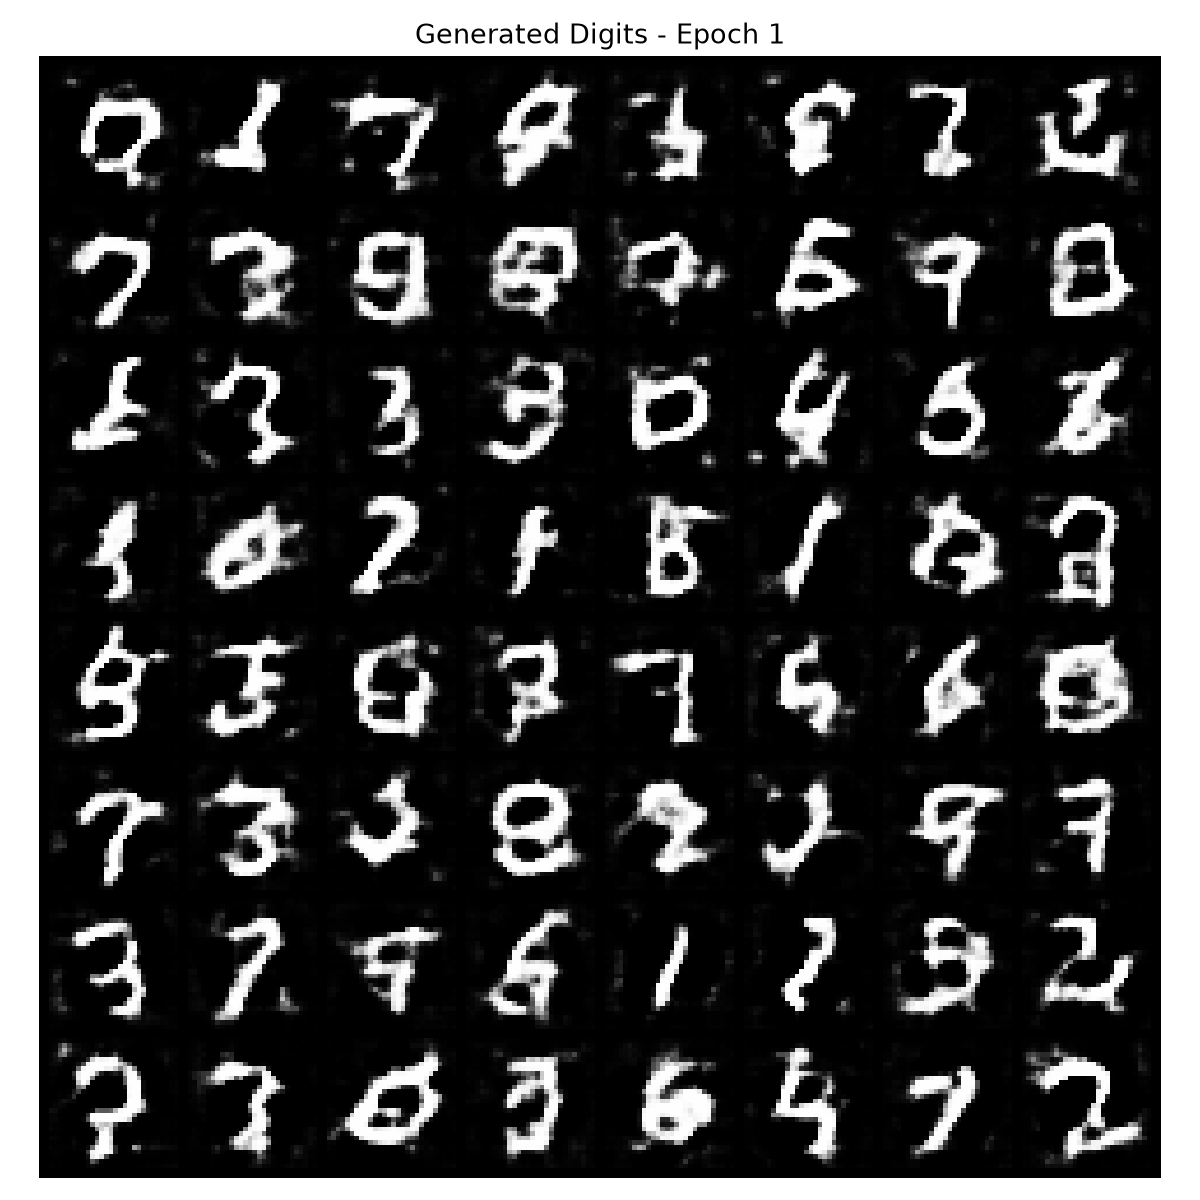
\includegraphics[width=0.6\textwidth]{outputs/samples/epoch_001.png}
    \caption{Generated samples at Epoch 1 --- random noise, no digit structure}
\end{figure}

\begin{figure}[H]
    \centering
    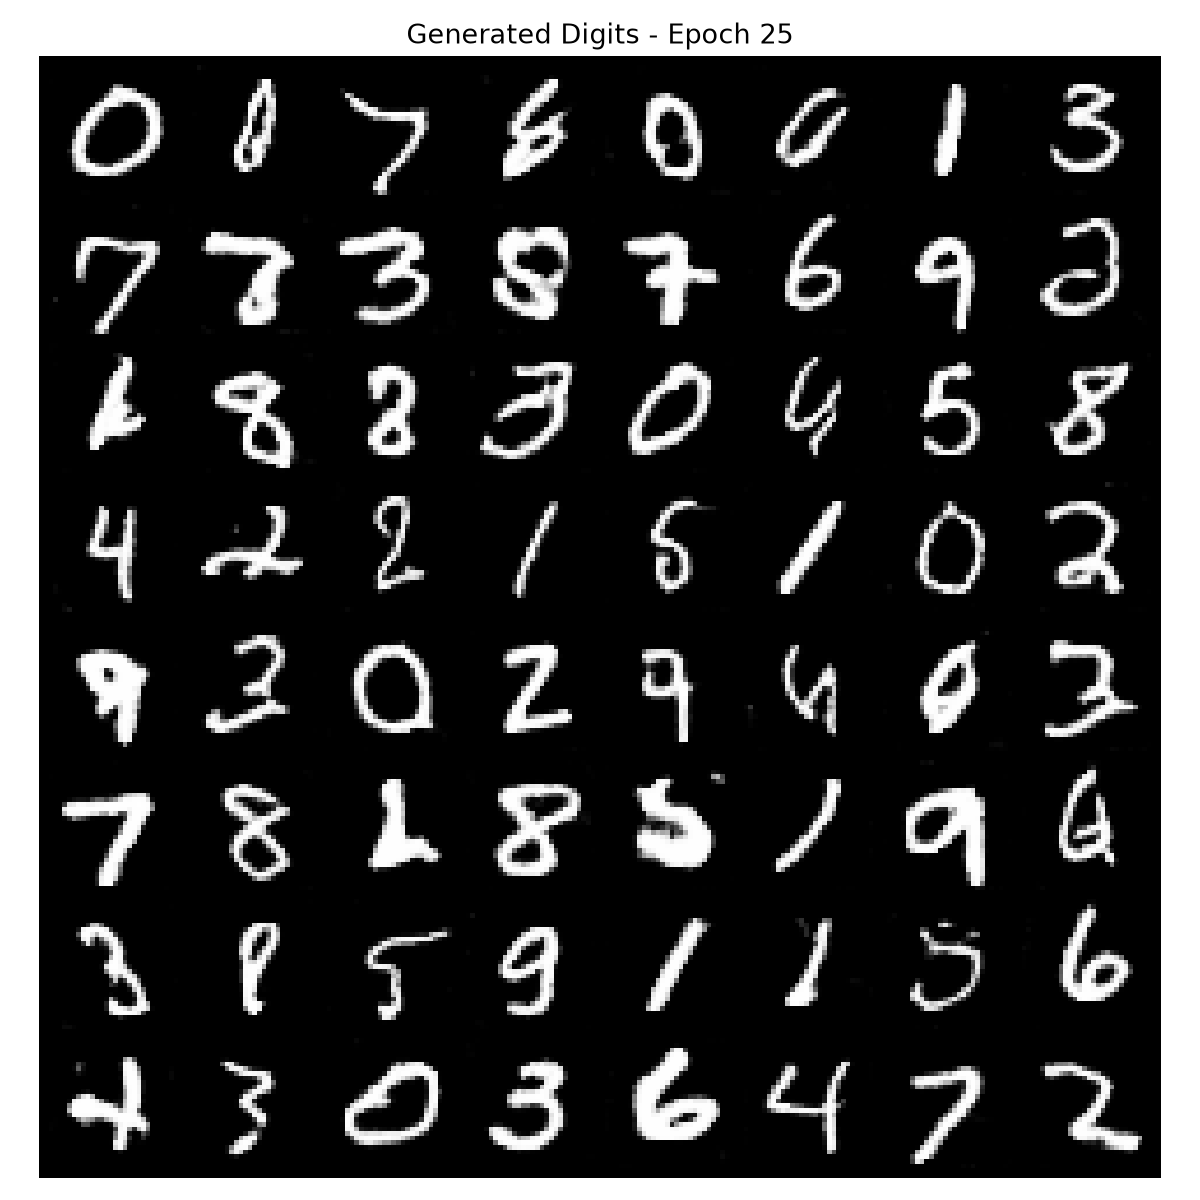
\includegraphics[width=0.6\textwidth]{outputs/samples/epoch_025.png}
    \caption{Generated samples at Epoch 25 --- recognisable digit-like shapes emerging}
\end{figure}

\begin{figure}[H]
    \centering
    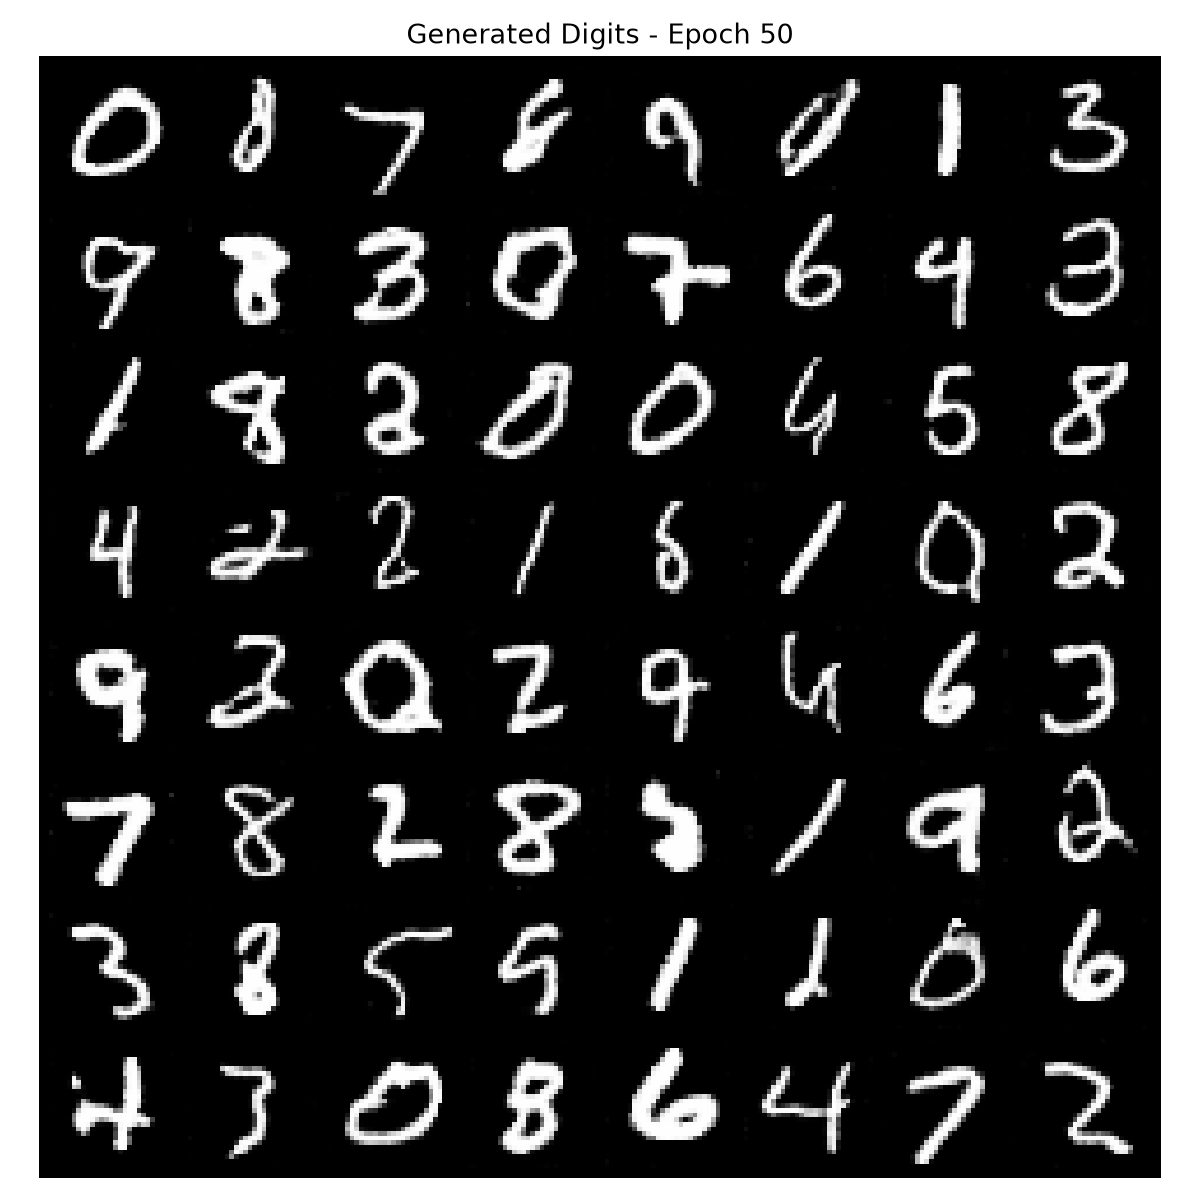
\includegraphics[width=0.6\textwidth]{outputs/samples/epoch_050.png}
    \caption{Generated samples at Epoch 50 --- legible handwritten digits}
\end{figure}

\begin{figure}[H]
    \centering
    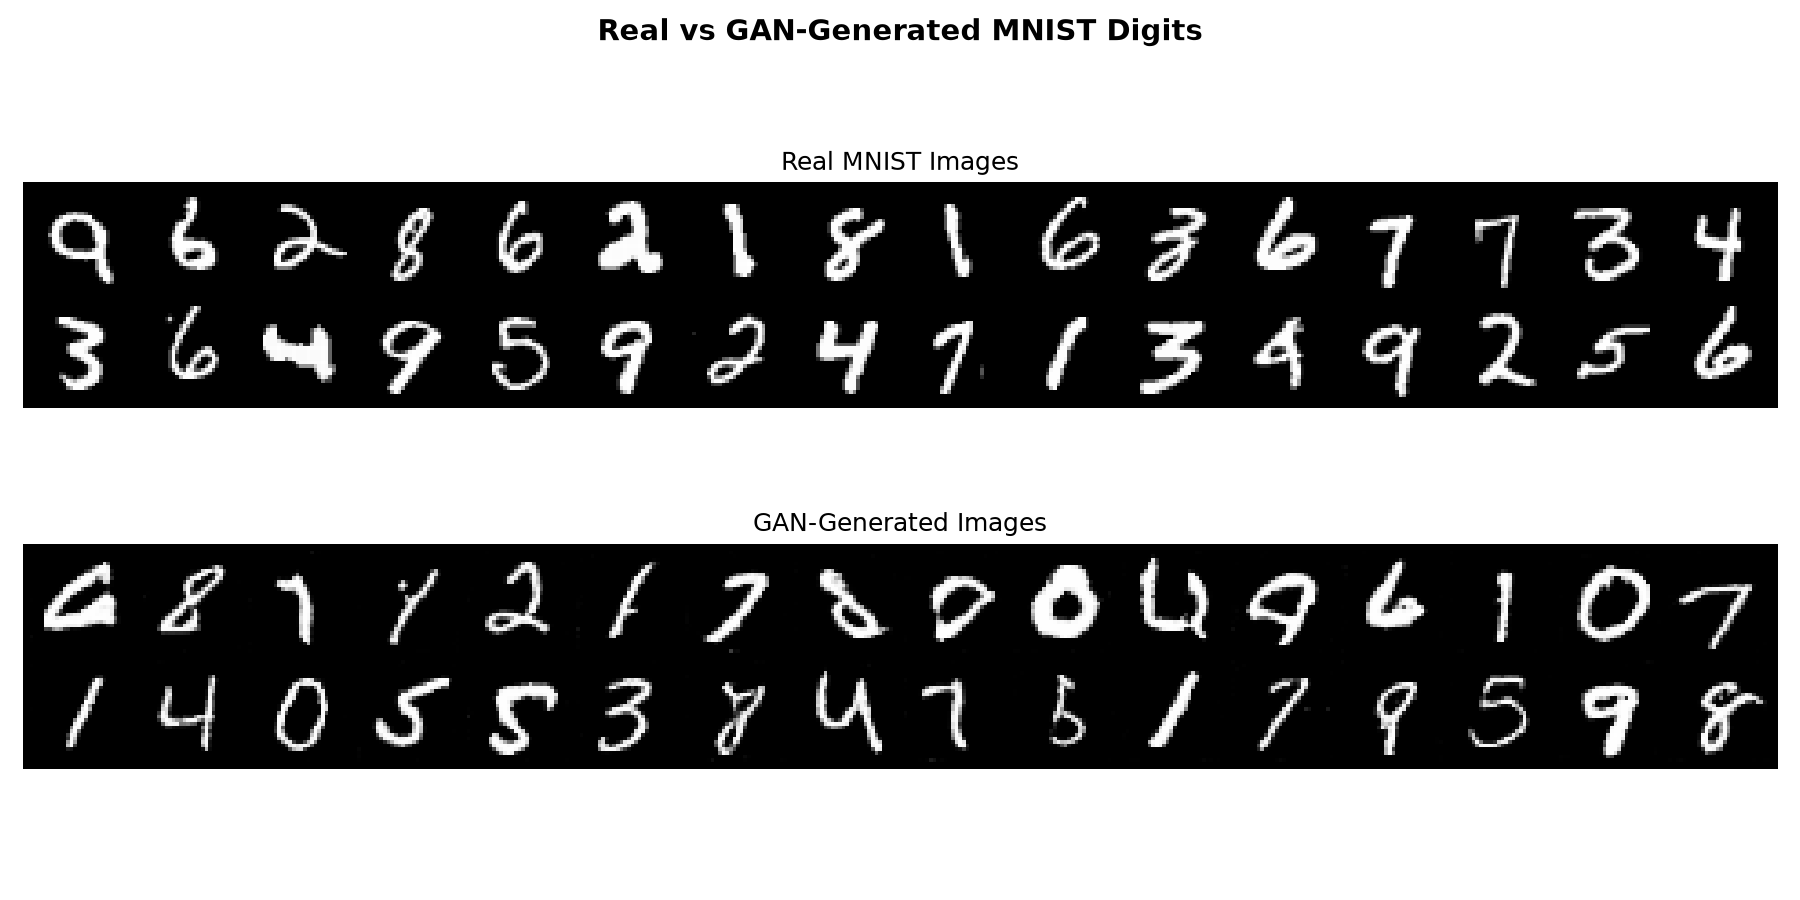
\includegraphics[width=\textwidth]{outputs/samples/real_vs_fake.png}
    \caption{Real MNIST images (top) vs GAN-generated images (bottom)}
\end{figure}

\begin{figure}[H]
    \centering
    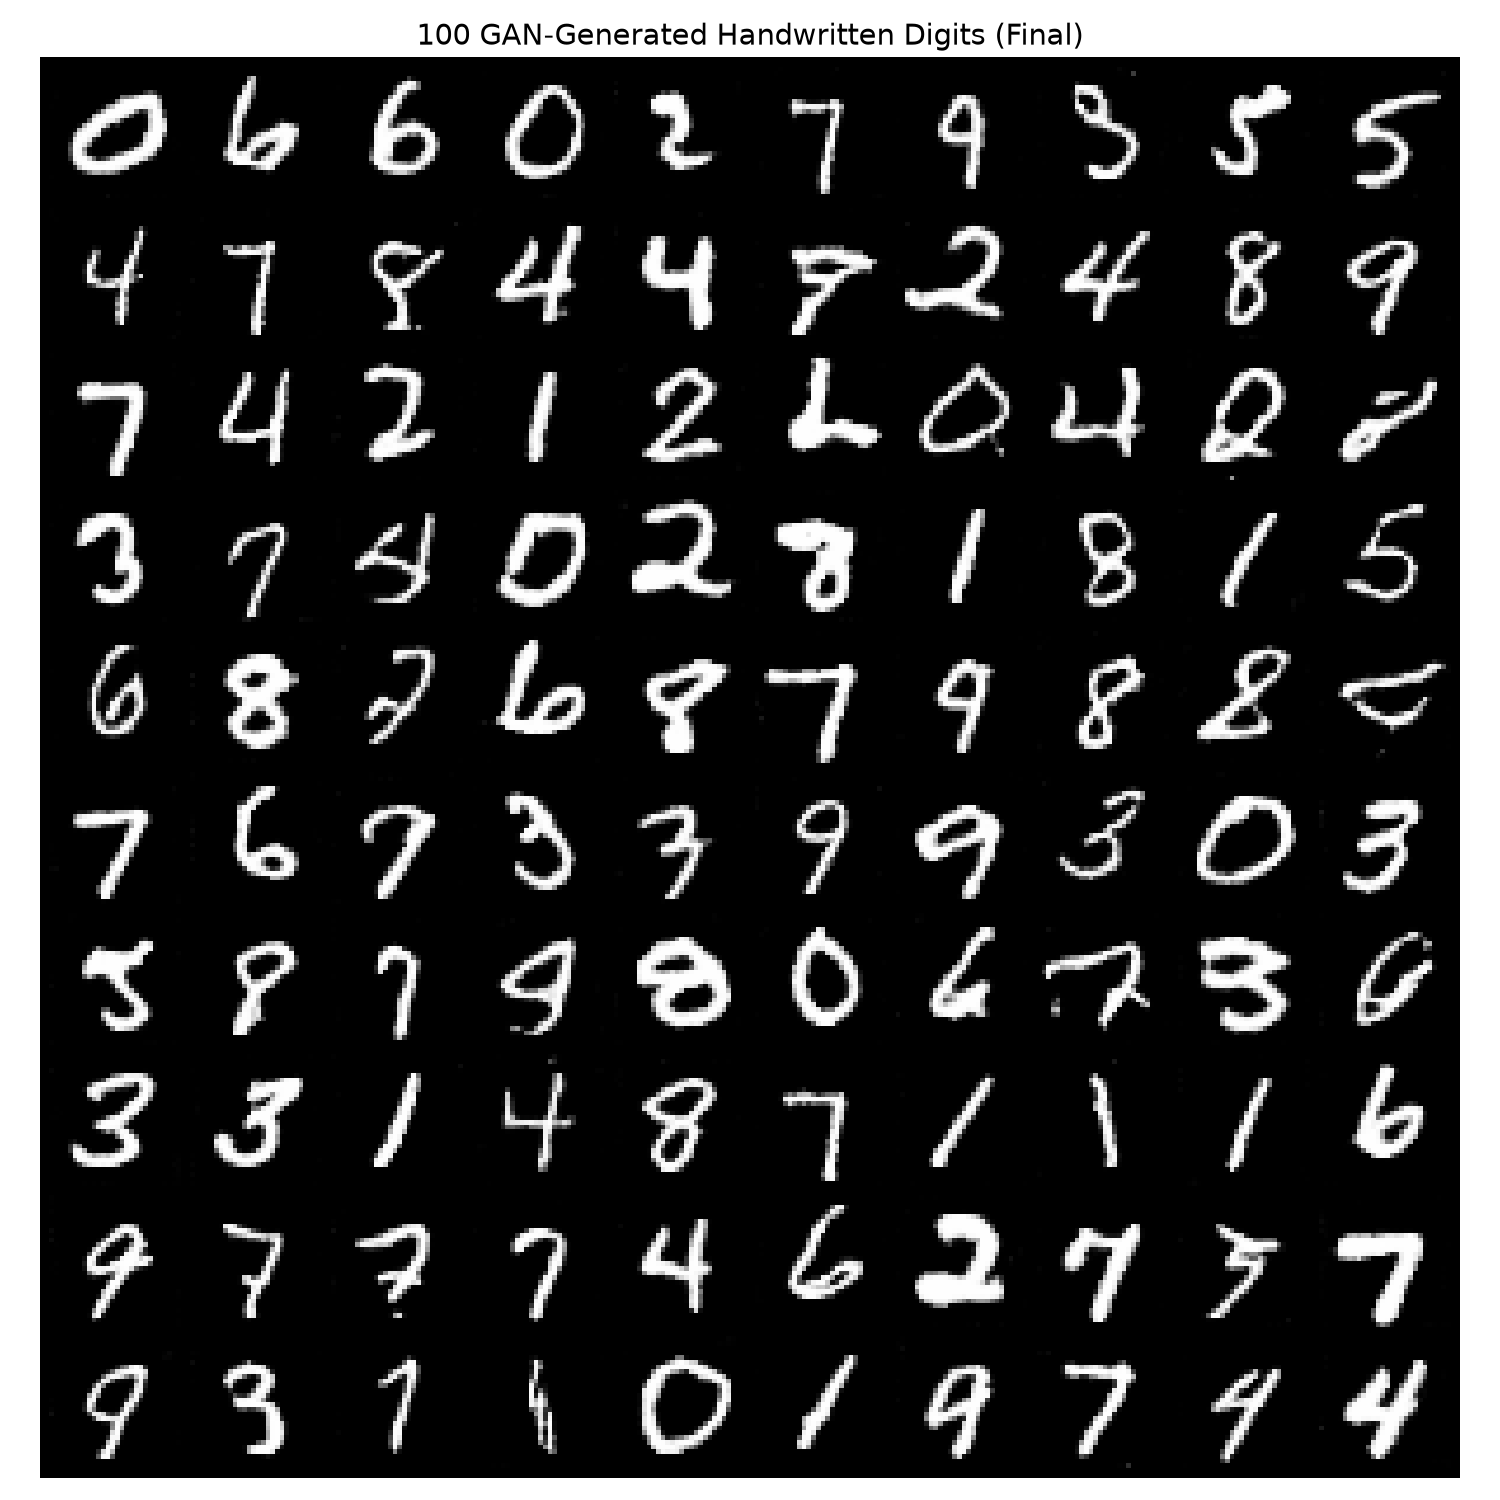
\includegraphics[width=0.8\textwidth]{outputs/samples/final_generated_100.png}
    \caption{100 GAN-generated handwritten digits from the final trained model}
\end{figure}

\subsection{Latent Space Interpolation}

To verify that the Generator has learned a structured representation rather than
memorising training examples, linear interpolation was performed between two random
noise vectors $\mathbf{z}_1$ and $\mathbf{z}_2$:

\begin{equation}
    \mathbf{z}_\alpha = (1 - \alpha)\,\mathbf{z}_1 + \alpha\,\mathbf{z}_2, \quad \alpha \in [0, 1]
\end{equation}

\begin{figure}[H]
    \centering
    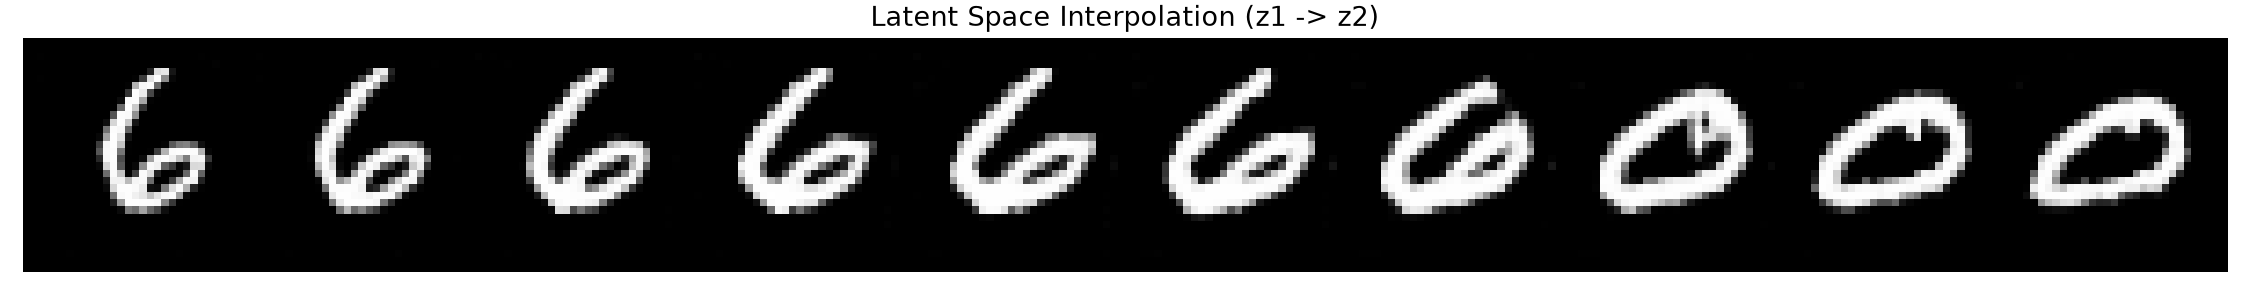
\includegraphics[width=\textwidth]{outputs/samples/latent_interpolation.png}
    \caption{Latent space interpolation from $\mathbf{z}_1$ to $\mathbf{z}_2$ in 10 steps}
\end{figure}

The smooth transitions between digit types confirm that the Generator has learned a
continuous, meaningful latent space. Intermediate images are plausible digits, not
incoherent noise.

\subsection{Limitations}

\begin{itemize}
    \item No quantitative metric such as FID (Fr\'{e}chet Inception Distance) was computed
          due to compute constraints.
    \item The fully-connected architecture produces slightly blurrier images than
          convolutional GANs (e.g.\ DCGAN), as it does not exploit spatial locality.
    \item The model generates digits without class control. A Conditional GAN (cGAN)
          would allow specifying which digit to generate.
\end{itemize}

% ─────────────────────────────────────────────────────────────────────────────
\section{Conclusion and Future Scope}

\subsection{Conclusion}

A fully-connected GAN was implemented and trained on MNIST over 50 epochs, successfully
learning to generate realistic synthetic handwritten digit images from 64-dimensional
Gaussian noise. The adversarial training dynamic converged to a stable equilibrium
(Generator loss: 1.6571, Discriminator loss: 0.9320), and the generated digits are
visually plausible across all ten digit classes. Latent space interpolation confirmed
that the model has learned a smooth, continuous internal representation of handwritten
digits rather than memorising training examples. The project validates the core GAN
principle: two competing networks, trained jointly, produce a generative model capable
of synthesising novel and realistic samples.

\subsection{Future Scope}

\begin{enumerate}
    \item \textbf{Conditional GAN (cGAN):} Condition on the digit class label to generate
          a specific digit on demand \cite{mirza2014}.
    \item \textbf{Wasserstein GAN (WGAN):} Replace BCE loss with the Wasserstein distance
          for more stable training and better convergence guarantees \cite{arjovsky2017}.
    \item \textbf{DCGAN:} Replace fully-connected layers with convolutional and transposed
          convolutional layers for sharper, higher-quality generated images \cite{radford2015}.
    \item \textbf{FID Score:} Compute Fr\'{e}chet Inception Distance for quantitative
          quality benchmarking.
    \item \textbf{Data Augmentation:} Use generated images to augment training data for
          digit classifiers on class-imbalanced datasets.
\end{enumerate}

% ─────────────────────────────────────────────────────────────────────────────
\begin{thebibliography}{99}

\bibitem{goodfellow2014}
I.\ Goodfellow, J.\ Pouget-Abadie, M.\ Mirza, B.\ Xu, D.\ Warde-Farley, S.\ Ozair,
A.\ Courville, and Y.\ Bengio,
``Generative Adversarial Nets,''
\textit{Advances in Neural Information Processing Systems (NeurIPS)}, 2014.

\bibitem{radford2015}
A.\ Radford, L.\ Metz, and S.\ Chintala,
``Unsupervised Representation Learning with Deep Convolutional Generative Adversarial Networks,''
\textit{arXiv preprint arXiv:1511.06434}, 2015.

\bibitem{lecun1998}
Y.\ LeCun, C.\ Cortes, and C.\ J.\ C.\ Burges,
``The MNIST Database of Handwritten Digits,''
1998. [Online]. Available: \url{http://yann.lecun.com/exdb/mnist/}

\bibitem{mirza2014}
M.\ Mirza and S.\ Osindero,
``Conditional Generative Adversarial Nets,''
\textit{arXiv preprint arXiv:1411.1784}, 2014.

\bibitem{arjovsky2017}
M.\ Arjovsky, S.\ Chintala, and L.\ Bottou,
``Wasserstein GAN,''
\textit{arXiv preprint arXiv:1701.07875}, 2017.

\bibitem{salimans2016}
T.\ Salimans, I.\ Goodfellow, W.\ Zaremba, V.\ Cheung, A.\ Radford, and X.\ Chen,
``Improved Techniques for Training GANs,''
\textit{Advances in Neural Information Processing Systems (NeurIPS)}, 2016.

\bibitem{kingma2013}
D.\ P.\ Kingma and M.\ Welling,
``Auto-Encoding Variational Bayes,''
\textit{arXiv preprint arXiv:1312.6114}, 2013.

\end{thebibliography}

\end{document}
